\chapter{Introduction}
In last few decades importance of computers in our everyday lifes has laregly increased.
A lot of us can only hardly imagine doing their jobs without help of appropriate computer program
and we also spend a plenty of time using computers (e.g. personal computers or mobile devices) in leisure time.
There is also wide usage of computers in more critical applications like autopilot in an aeroplane
or programs for controlling power stations.
But growing number of applications of computer programs brings also need for their safety and security.

However, guarantee of software quality and correctness is not easy task
because programs has often many state which they go through during computation
and it could be very time and (memory) space demanding to check whether no undesirable thing
happens in any of the visited states.
One approach to ensure software qaulity is \emph{testing} (and dynamic analysis) which is basically based
on runnig a program in the different contexts and under the different inputs
and checking whether programs behaviour and outputs are expected one.
This method can satisfy many of requiremnts for software quality and often cover greate space of programs behaviours
but on the other side it is only possbile to prove presence of the errors using testing not their absence (\cite{djikstra}).
Moreover finding errors during testing does not mean that all of them has been found.

The mentioned weakness of testing can be resolved by \emph{formal verification}
which is another approach to checking program correctness.
Formal verification is method for checking whether a given system meets a given specification \cite{fav:lecture}.
There are three main branches of formal verification.
The first one is \emph{model checking} which systematically explores of a model (e.g. model of a program) to
prove that a property holds along the whole model.
The second approach is static analysis which is done over a source code (or some modification of it) of a system
without its explicit execution.
The last one is \emph{theorem proving}.
It proves the program in standard mathematical way -- starting from axioms and proving theorems to
verify the properties of a given system.
Theorem proving could be more or less automated.

This thesis deals with specific part of static analysis called shape analysis which is focused to verification of the programs manipulating
complex data structures (like a different kinds of lists and trees) allocated on the heap.
The properties checked for this class of programs are for example checking whether no dangling
pointers are dereferenced (no invalid dereference), whether all allocated memory on a heap is also freed (no memory leaks)
a program exuction or whether there is not dealocated pointer which has not have assigned memory (no invalid free).
There are different approaches to this kind of static analysis with the different advantages.
For example approach based on \emph{seperation logic} brings scalability to a verification procedure.
On the other side, automata based approach, conceretly \emph{abstract tree regular model checking}, is
superior in flexibility.
However, this theisis will be focused to a verification procedure employing concept of Forest automata (FA) which tries
to synthetize benefits of the mentioned approaches.

Forest automata has been introduce in \cite{forester} and they are extension of finite automata or more precisly finite tree automata.
They are used as abstract domain in this verification procedure.
Basically, the verification procudere based on FA is perforing symbolic execution of a verified program and
FA serves here as the abstract domain.
A prototype of this verification procedure has been implemented in tool called \emph{Forester}.
Forester verifies programs in language C and it can detect invalid dereferences, invalid free, memory leaks and also reachability of an error label.
It is yet able to verify non-trivial data structures like skiplist of the second and the third level
but there is still room for improvement, e.g. by extending support of C language.

The main topic of this topic is improvement of Forester tool.
Since FA are highly related to finite tree automata (TA) the first of goal is to connect
Forester with VATA library -- state-of-the-art library for TA manipulation \cite{tacas12}.
Particulary, this consists creating of an interface between Forester and VATA to employ VATA as TA library for Forester backend.
The second goal of this thesis is to implement \emph{backward run} for Forester what enables checking spuriousness of an error found in program.
The error could be spurous because of used to high abstraction over FA domain but the information get by backward could be used for refinment of \emph{predicate abstraction}
what is one kind of abstraction used in Forester (another one is \emph{height abstraction}.
It was also not possible to fully test predicate abstraction because of absence of backward run implementation
so a part of this goal is to complete and test implementation of predicate abstraction.

A structure of this theisi will be following.
In Chapter \ref{ch:prel} will be given definitions of preliminaries for further text.
Chapter \ref{ch:tools} provides description of VATA library and Forester tool.
General principle of backward run and predicate abstract is given in Chapter \label{ch:pred} and their
application for verification based on FA is described in Chapter \label{ch:backwar}.
Chapter \ref{ch:impl} provides description of implementation and finally Chapter \ref{ch:eval} is about evalutation.
\cite{Knuth}

\chapter{Preliminaries}
\label{ch:prel}

This chapter gives the definitions of the basic concepts.
First, the graphs, trees and forests are defined together with automata accepting them in Section \ref{sec:graph}.
Then the forest automata are extended to the forest automata of higher level in Section \ref{sec:fah}.
This section follow the definitions and a structure used in \cite{cav13:techrep}.

\section{Graphs, Trees and Forests}
\label{sec:graph}

Let us suppose a word $w = a_1 \ldots a_n$, we denote $i$-th symbol of $w$ as $a_i$.
We denote $dom(f)$ domain of a total mapping $\funcdecl{f}{A}{B}$ and its range is denoted by $rng(f)$.

\subsection{Graphs and Trees}
\label{subsec:graph}
A \emph{ranked alphabet} is a finite set of symbols $\Sigma$ and a related mapping $\funcdecl{\#}{\Sigma}{\mathbb{N}}$
assigning to a symbol its rank.
A (directed, ordered, labelled) \emph{graph} is a total map $\funcdecl{g}{V}{\Sigma \times V^{*}}$ where $V$ is a finite set of nodes.
The items of set $\Sigma$ are within graph context called \emph{labels}.
Map $g$ maps each node $v\in V$ to:
\begin{enumerate}
	\item A label $\alpha \in \Sigma$ that we will denote by $l_g(v)$.
	\item A sequence of \emph{successors} $(v_1 \cdots v_n) \in V^n$ for a $n \in \mathbb{N}$.
		We denote successors by $S_g(v)$ and $v_i$ is denoted by $S^i_g(v)$.
\end{enumerate}
It holds that $\#(l_g(v)) = |S_g(v)|$.
We will omit subscript $g$ when no ambiguity is possible.

A \emph{leave} of $g$ is a node $v \in V$ such that $S_g(v) = \epsilon$.
An \emph{edge} of $g$ is a pair $v \mapsto (a, v_1 \cdots v_n))$ where $v, v_1, \ldots, v_n \in V$,
$a \in \Sigma$ such that $g(v) = (a, v_1 \cdots v_n)$.
\emph{In-degree} of a node $v' \in V$ in graph $g$ is the overall number of occurrences in $g(v)$ for any $v \in V$.
We will in-degre of a node $v \in V$ by $idg_g(v)$ and we will again omit subscript $g$ whenever it is possible.
More formal, in-degree is defined as $idg(v') = |\{v \mapsto (a, v_1 \cdots v_n)) \emph{ is an edge such that } \exists i \in \{1,\ldots,n\}: v' = v_i\}|$.
The \emph{joins} of $g$ are nodes $v \in V$ such that $idg(v') > 1$.

A \emph{path} from $v\in V$ to $v' \in V$ is a sequence $p=v_0, i_1, v_1, \ldots, i_n, v_n$ where $v=v_0, v' = v_n$
and $\forall j \in \{1,\ldots,n\}: v_j = S^{i_j}(v_{j-1})$ (informally, $v_j$ is the $i^j$-th successor of $v_{j-1}$).
A empty path has $n=0$.
A node $u \in V$ is \emph{reachable} from a node $v \in V$ iff that is a path from $v$ to $u$ or $u=v$.
A node $u \in V$ is \emph{root} of $g$ iff all nodes $v \in V$ are reachable from $u$.
We will use term $root$ also for a mapping $\funcdecl{root}{g}{V}$ which maps a graph to its root.
When there is a root in a graph then the graph is called \emph{rooted}.

A \emph{tree} $t$ is a graph which is either empty, or it has exactly one root and $\forall v \in V: idg(v) <= 1$ (informally,
each node is a successor of at most one of the other nodes).

\subsection{Forests}
\label{subsec:forests}

Let us suppose withou loss of generality that $\Sigma \cap \mathbb{N} = \emptyset$.
A $\Sigma$-labelled \emph{forest} is a sequence of tree $t_1, \ldots, t_n$ over ($\Sigma \cup \{1,\ldots,n\}$)
where $\forall i \in \{1,\ldots,n\}: \#i = 0$.
\emph{Root preferences} are leaves labelled $i \in \mathbb{N}$.
The forest $t_1,\ldots,t_n$ (we suppose that their nodes sets are disjoint) represents the graph $\fagr$ that could
be constructed by interconnecting their roots with the related root reference.
E.g. when there is a root reference $2$ in $t_1$ then this leaf is replaced by the root node of $t_2$.
Let's formalize the idea of construction of $\fagr$.
$\fagr$ contains an edge $v \mapsto (a,v_1, \ldots,v_m)$ iff $\exists i \in \{1,\ldots,n\} \ \exists(v \mapsto (a, v_1', \ldots, v_m')) \in edges(t_i)
\ \forall j \in \{1,\ldots,m\}: v_j = h(v_j')$ where $edges(t_i)$ is the set of all edges of a tree $t_i$ and
\[ h(v_j') = \left\{
  \begin{array}{l l}
  root(t_k) & \quad \text{if $v_j'$ is a root reference with $l(v_j') = k$}\\
  v_j'   & \quad \text{otherwise}
  \end{array} \right.\]

TODO Canonicity

\subsection{Graphs and Forests with Ports}

We will extend graphs and forests with concept of the \emph{ports} which should
serve for marking input and output nodes.
An \emph{input-output-graph} (io-graph) is a pair $(g,\phi)$ (in sense of brevity also denoted by $g_\phi$)
where $g$ is a graph and $\phi=(\phi_1 \cdots \phi_n) \in dom(g)^+$ is a sequence of ports, $\phi_1$
is an input port and $\phi_1 \cdots \phi_n$ is a sequence of output ports.
The ports in $\phi$ are unique.
If a root if $g_\phi$ is $\phi_1$ then $g_\phi$ is \emph{accessible}.

The \emph{cut-points} of a graph $g_\phi$ is the set of its ports and joins and we denote this set by $cps(g_\phi)$.
Formally, $cps(g_\phi)=\{v \in V\,|\, v \in \phi \vee idg(v) > 1\}$.

An \emph{io-forest} is a pair $f=(t_1 \cdots t_n, \pi)$ such that $n \geq 1$ and $\pi \in \{1,\ldots,n\}^n$
is a sequence of port indicies, where $\pi_1$ is the input port index and $\pi_2 \ldots \pi_{|\pi|}$ is a sequence
of the output ports indicies.
The indicies are unique as in the case of ports.
It is also possible to construct a io-graph $\otimes f$ from a forest $f$ such that
$\otimes f = (\otimes t_1 \cdots t_n,root(t_{\pi_{1}},\ldots,t_{\pi_{n}}))$.
So the port of $\otimes f$ are roots of the trees indexed by indicies in $\pi$.
This means that a root of tree pointed by $\pi_1$ is an input port of $\otimes f$ and
the roots of trees pointed by the other indicies in $\pi$ are the output ports of $\otimes f$.

\subsection{Tree Automata}
\label{subsec:ta}

A (finite, non-deterministic, top-down) \emph{tree automaton} (TA) is a
quadruple $A = (Q, \Sigma, \Delta, R)$ where
\begin{itemize}
	\item $Q$ is a finite set of \emph{states}
	\item $\Sigma$ is a ranked alphabet
	\item $\Delta$ is a set of \emph{transition rules} where transition has a form $(q,a,q_1 \cdots q_n)$ where $q,q_1,\ldots,q_n \in Q$, $a \in \Sigma$, $n \geq 0$ and $\#a = n$.
		Alternatively, we write $q \xrightarrow{a} (q_1 \cdots q_n)$ to denote a $(q,a,q_1 \cdots q_n) \in \Delta$.
		When $n=0$ then the rule is called \emph{leaf rule}.
	\item $R \subseteq Q$ is a set of \emph{root states}.
\end{itemize}

We could symetrically define also bottom-up tree automata as quadruple $B = (Q, \sigma, \Delta, F)$ where
\begin{itemize}
	\item $Q$ is a finite set of states
	\item $\Sigma$ is a ranked alphabet
	\item $\Delta$ is a set of transition rules where transition has a form $(q_1 \cdots q_n,a,q)$ where $q,q_1,\ldots,q_n \in Q$, $a \in \Sigma$, $n \geq 0$ and $\#a = n$.
		We can again write $(q_1 \cdots q_n) \xrightarrow{a} q$ to denote a $(q_1 \cdots q_n,a,q) \in \Delta$.
		When $n=0$ then the rule is called \emph{leaf rule}.
	\item $F \subseteq Q$ is a set of \emph{final states}.
\end{itemize}

We will further consider top-down tree automata as default.

Since syntax of a TA is already defined we are going to define its semantics.
A \emph{run} of a TA $A$ over a tree $t$ is mapping $\funcdecl{\rho}{dom(t)}{Q}$ such that
$\forall v \in dom(t)\ \exists (q \xrightarrow{a} (q_1 \cdots q_n)) \in \Delta:  q=\rho(v) \wedge  \forall i \in \{1, \ldots, |S(v)|\}: q_i=\rho(S(v)_i)$.
We use $t \Rightarrow_{\rho} q$ to denote a run $\rho$ of TA A over tree $t$ s.t. $\rho(t) = q$ and we use $t \Rightarrow q$ to denote that there exists
a run $\rho$ over $t$ to $q$.
Finally, we can define language of a TA.
The \emph{language} of a state $q\in Q$ is defined by $L(q) = \{t\,|\, t \Rightarrow q\}$.
The \emph{language} of a NTA $A$ is defined by $L(A) = \Cup_{q\in R} L(q)$.

\subsection{Forest Automata}
\label{subsec:fa}

A \emph{Forest Automata} (FA) over $\Sigma$ is a pair $F=(A_1\cdots A_n, \pi)$
where $A_1 \cdots A_n$ is a sequence of tree automata defined over alphabet $\Sigma \cup \{1,\ldots,n\}$
and $\pi = I_1 \cdots I_n$ where $I_1,\ldots, I_n \in \{1, \ldots, n\}$ is a sequence of port indicies.
There are two kinds of languages related to FA.
The first one is forest langauge obtained by cartesian product of the languages of particular TA (and port indicies) of FA
what gives a set of io-forests.
The second one is graph language obtained by uniting of the io-forests from forest language to a io-graph.
Formally, The \emph{forest language} of the FA $F$ is the set of io-forests $L_f(F)= L(A_1) \times \ldots L(A_n) \times \{\pi\}$.
Please note that it is neccessary to add to the cartesian product also sequence of indicies to preseve structure of io-forests
and so to be able to construct graph language of $F$.
The \emph{graph language} of $F$ is the set of io-graph $L(F) = \{\times f\,|\, f \in L_f{F}\}$.

TODO inclusion and canonicity

\section{Forest Automata of Higher Level}
\label{sec:fah}

\subsection{Structured Labels}

\subsection{Forest Automata of Higher Level}

\chapter{Forest Automata based Verification}
\label{ch:fav}

\chapter{\vata\ and Forester}
\label{ch:tools}

As it was mentioned in introduction, FA based verification is implemented by tool
called Forester.
Since the FA are closely related to TA as it was shown in Chapter \ref{ch:prel} so
Forester also depends on an implementation of TA.
It currently has its own implementation of TA providing operations over TA needed during verification procedure.
However it is quite impratical to mantain a special TA library inside of Forester
and it would be more practical to employ some existing efficient TA library.
One very efficient library is the VATA library which provides implementation of standard operations over TA like union or intersection
but it also implements state-of-the-art algorithms \cite{tacas11} for language inclusion checking which efficiency
is also crucial for performance of Forester.
It seems logical according to these facts to connect Forester with the VATA library employing VATA like a backend TA library for Forester.

This chapter will provide a description of the VATA library firstly and then also a description of Forester.
Finally the implementation of Forester using VATA library done as a part of this thesis will be described.

\section{\vata}
\label{sec:VATA}

\vata\ is open source library for nondeterministic tree automata.
Its main application is in the field of formal verification.
VATA is licensed under GPL, version 3, and can be obtained from its official website \cite{www:vata}.
Implentation programming language is C++.
It is the only library to our knowledge implementing state-of-the algorithms for checking inclusion of NTA languages
what makes it suitable for usage as a Forester backend library.
However, \vata\ does not only provide implementation of algorithms for NTA but also highly efficient implementation of
algorithms for nondeterministic finite automata \cite{hruska13}.

\subsection{Design}
\vata\ currently provides methods for representation of NTA in explicit encoding and also in semi-symbolic (top-down and bottom-up)
encoding using \emph{MTBDD} but it has been designed to be easy extended by other encodings (for others automata).
The library provides both API for creating and manipulating NTA to other programs and also command line interface (cli) build around
the API for experimenting with tree automata in text format directly from command line.
The main idea of the design of the library is given in Figure \ref{fig:vata}.
As you can see there are the three main parts in the library design:
\begin{enumerate}
	\item \emph{Parsers} -- Parsing an input automaton from a text file.
		Timbuk \cite{timbuk} is currently the only one supported format for parsing input automata.
	\item \emph{Serializers} -- Serializing an automaton to a text file.
		Timbuk format is again the only one supported format.
	\item \emph{Automata encodings} -- The particular encodings of NTA.
		An encoding should consists of core module implementing of NTA representation itself
		and also the operations over NTA in this encoding.
\end{enumerate}

\begin{figure}[bt]
\begin{center}
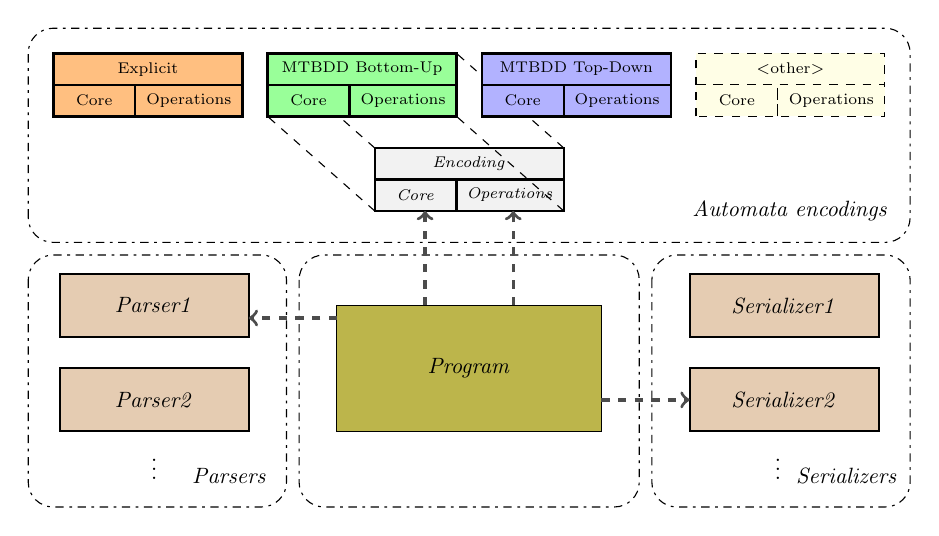
\begin{tikzpicture}
[
  scale=1,
  transform shape,
	gen/.style={thick,fill=gray!10},
	expl/.style={thick,fill=orange!50},
	bu/.style={thick,fill=green!40},
	td/.style={thick,fill=blue!30},
	other/.style={fill=yellow!10,dashed}
]

% encodings
\draw[dashed] (0,1) -- (-1.7,2.5);
\draw[dashed] (0,0) -- (-1.7,1.5);
\draw[dashed] (3,1) -- (1.3,2.5);

\draw (0,0.5) rectangle +(3, 0.5) [gen] node[midway] {\textit{\scriptsize{Encoding}}};
\draw (0,0) rectangle +(1.3, 0.5) [gen] node[midway] {\textit{\scriptsize{Core}}};
\draw (1.3,0) rectangle +(1.7, 0.5) [gen] node[midway] {\textit{\scriptsize{Operations}}};

\draw (-5.1,2) rectangle +(3, 0.5) [expl] node[midway] {\scriptsize{Explicit}};
\draw (-5.1,1.5) rectangle +(1.3, 0.5) [expl] node[midway] {\scriptsize{Core}};
\draw (-3.8,1.5) rectangle +(1.7, 0.5) [expl] node[midway] {\scriptsize{Operations}};

\draw (-1.7,2) rectangle +(3, 0.5) [bu] node[midway] {\scriptsize{MTBDD Bottom-Up}};
\draw (-1.7,1.5) rectangle +(1.3, 0.5) [bu] node[midway] {\scriptsize{Core}};
\draw (-0.4,1.5) rectangle +(1.7, 0.5) [bu] node[midway] {\scriptsize{Operations}};

\draw (1.7,2) rectangle +(3, 0.5) [td] node[midway] {\scriptsize{MTBDD Top-Down}};
\draw (1.7,1.5) rectangle +(1.3, 0.5) [td] node[midway] {\scriptsize{Core}};
\draw (3.0,1.5) rectangle +(1.7, 0.5) [td] node[midway] {\scriptsize{Operations}};

\draw (5.1,2) rectangle +(3, 0.5) [other] node[midway] {\scriptsize{$<$other$>$}};
\draw (5.1,1.5) rectangle +(1.3, 0.5) [other] node[midway] {\scriptsize{Core}};
\draw (6.4,1.5) rectangle +(1.7, 0.5) [other] node[midway] {\scriptsize{Operations}};

\draw[dashed] (3,0) -- (1.3,1.5);

\draw[rounded corners=9,dash pattern=on 3pt off 2pt on 1pt off 2pt] (-5.5,-0.5) rectangle +(14,3.4);

\draw (6.6,0) node {\textit{Automata encodings}};


% parsers
\draw (-5,-2) rectangle +(3, 1) [gen,fill=brown!40] node[midway] (parser1) {\textit{Parser1}};
\draw (-5,-3.5) rectangle +(3, 1) [gen,fill=brown!40] node[midway] {\textit{Parser2}};
\draw (-3.5,-4) node {$\vdots$};

\draw[rounded corners=9,dash pattern=on 3pt off 2pt on 1pt off 2pt] (-5.5,-0.7) rectangle +(4.1,-4);
\draw (-2.3,-4.2) node {\textit{Parsers}};

% serializers
\draw (5,-2) rectangle +(3, 1) [gen,fill=brown!40] node[midway] {\textit{Serializer1}};
\draw (5,-3.5) rectangle +(3, 1) [gen,fill=brown!40] node[midway] {\textit{Serializer2}};
\draw (6.4,-4) node {$\vdots$};

\draw[rounded corners=9,dash pattern=on 3pt off 2pt on 1pt off 2pt] (4.4,-0.7) rectangle +(4.1,-4);
\draw (7.5,-4.2) node {\textit{Serializers}};

% program
\draw[rounded corners=9,dash pattern=on 3pt off 2pt on 1pt off 2pt] (-1.2,-0.7) rectangle +(5.4,-4);

\draw[fill=olive!60] (-0.6,-1.5) rectangle (3.6,-3.5) node[midway] {\textit{Program}};

\draw[very thick,dashed,->,black!70] (-0.6,-1.7) -- (-2,-1.7);
\draw[very thick,dashed,->,black!70] (3.6,-3) -- (5,-3);
\draw[very thick,dashed,->,black!70] (0.8,-1.5) -- (0.8,0);
\draw[very thick,dashed,->,black!70] (2.2,-1.5) -- (2.2,0);

\end{tikzpicture}

		\caption{The main concept of \vata. Figure is taken from \cite{tacas12}}.
		\label{fig:vata}
\end{center}
\end{figure}

A \emph{program} (e.g. cli of VATA is such a program) employing the three parts of \vata\ could works as follows.
An input automaton is loaded by one of the parsers to an intermediate representation.
The wrapping program chooses internal encoding of NTA to which is automaton stored from intermediate encoding (please note that it is also
create automaton in the chosen enconding directly using API provided by VATA).
Then the automaton is processed and the applied operations are implemented by module of the chosen encoding.
Finally, automaton could be serialized to an output format.
When one wants to add her own encoding then she needs to implement only core of encoding (with API for creating automaton itself)
and ofcourse needed operations and can employ already implemented parses and serializers of \vata.

\subsection{Implemented NTA encodings}

Using \emph{explicit enconding} NTA transition relation is represented by a hiearchy of the hash tables as it is shown in Figure \ref{fig:explnta}.
The first level of the hash tables hiearchy (\emph{top-level lookup tables}) maps each state $q$ of an automaton to 
a second level of the hash tables hiearchy (\emph{transition cluster}) where are store all symbols which
are presented in a transition where $q$ is at left-handed side.
Each symbol $a$ in a transition cluster is mapped to a pointer to a set in the third level of hiearchy (\emph{sets of pointers to tuples}).
The set contains pointers to tuples which are at right-handed side in a transition with $q$ at left-handed side and with $a$ as a symbol.
The tuples are stored at a special set where every tuples is stored only once.
Please note, that it also possible to share part of transition relation between different automata what
brings higher efficiency in space complexity of implementation.
Module for explicit encoding also stores explicitly set of the final states of a NFA but on
the other side it does not store anywhere explicitly set of states because it can be obtained from a transition relation.

\begin{figure}[bt]
\begin{center}
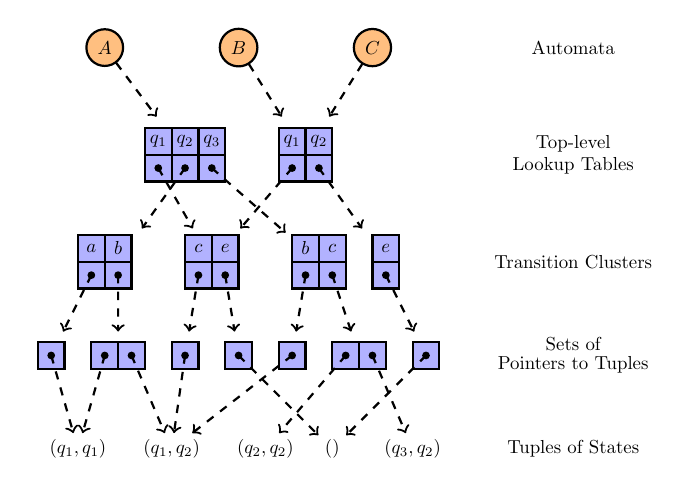
\begin{tikzpicture}
[
  scale=0.85,
  transform shape,
	gen/.style={thick,fill=gray!10},
	expl/.style={thick,fill=orange!50},
	bu/.style={thick,fill=green!40},
	td/.style={thick,fill=blue!30},
	other/.style={fill=yellow!10,dashed}
]

\node at(10,2) {Automata};

\node[expl,circle,draw] (aA) at(1.25,2) {\textit{$A$}};
\node[expl,circle,draw] (aB) at(3.75,2) {\textit{$B$}};
\node[expl,circle,draw] (aC) at(6.25,2) {\textit{$C$}};


\node at(10,0) {\shortstack{Top-level\\ Lookup Tables}};

\node[minimum size=40pt](table1) at (2.75,0) {};
\draw (2,0) rectangle +(0.5, .5) [td] node[midway] {\textit{$q_1$}};
\draw (2,-.5) rectangle +(0.5, .5) [td] node[midway] {};
\draw (2.5,0) rectangle +(0.5, .5) [td] node[midway] {\textit{$q_2$}};
\draw (2.5,-.5) rectangle +(0.5, .5) [td] node[midway] {};
\draw (3,0) rectangle +(0.5, .5) [td] node[midway] {\textit{$q_3$}};
\draw (3,-.5) rectangle +(0.5, .5) [td] node[midway] {};

\node[minimum size=40pt](table2) at (5,0) {};
\draw (4.5,0) rectangle +(0.5, .5) [td] node[midway] {\textit{$q_1$}};
\draw (4.5,-.5) rectangle +(0.5, .5) [td] node[midway] {};
\draw (5,0) rectangle +(0.5, .5) [td] node[midway] {\textit{$q_2$}};
\draw (5,-.5) rectangle +(0.5, .5) [td] node[midway] {};


\draw[->,thick,dashed] (aA) -- (table1);
\draw[->,thick,dashed] (aB) -- (table2);
\draw[->,thick,dashed] (aC) -- (table2);


\node at(10,-2) {Transition Clusters};

\node[minimum size=35](cluster1) at (1.5,-2) {};
\draw (0.75,-2) rectangle +(0.5, .5) [td] node[midway] {\textit{$a$}};
\draw (0.75,-2.5) rectangle +(0.5, .5) [td] node[midway] {};
\draw (1.25,-2) rectangle +(0.5, .5) [td] node[midway] {\textit{$b$}};
\draw (1.25,-2.5) rectangle +(0.5, .5) [td] node[midway] {};

\node[minimum size=35pt](cluster2) at (3.25,-2) {};
\draw (2.75,-2) rectangle +(0.5, .5) [td] node[midway] {\textit{$c$}};
\draw (2.75,-2.5) rectangle +(0.5, .5) [td] node[midway] {};
\draw (3.25,-2) rectangle +(0.5, .5) [td] node[midway] {\textit{$e$}};
\draw (3.25,-2.5) rectangle +(0.5, .5) [td] node[midway] {};

\node[minimum size=35pt](cluster3) at (5.25,-2) {};
\draw (4.75,-2) rectangle +(0.5, .5) [td] node[midway] {\textit{$b$}};
\draw (4.75,-2.5) rectangle +(0.5, .5) [td] node[midway] {};
\draw (5.25,-2) rectangle +(0.5, .5) [td] node[midway] {\textit{$c$}};
\draw (5.25,-2.5) rectangle +(0.5, .5) [td] node[midway] {};

\node[minimum size=35pt](cluster4) at (6.5,-2) {};
\draw (6.25,-2) rectangle +(0.5, .5) [td] node[midway] {\textit{$e$}};
\draw (6.25,-2.5) rectangle +(0.5, .5) [td] node[midway] {};


\draw[thick,fill=black] (2.25,-0.25) circle (0.5mm);
\draw[->,thick,dashed] (2.25,-.25) -- (cluster2);

\draw[thick,fill=black] (2.75,-0.25) circle (0.5mm);
\draw[->,thick,dashed] (2.75,-.25) -- (cluster1);

\draw[thick,fill=black] (3.25,-0.25) circle (0.5mm);
\draw[->,thick,dashed] (3.25,-.25) -- (cluster3);

\draw[thick,fill=black] (4.75,-0.25) circle (0.5mm);
\draw[->,thick,dashed] (4.75,-.25) -- (cluster2);

\draw[thick,fill=black] (5.25,-0.25) circle (0.5mm);
\draw[->,thick,dashed] (5.25,-.25) -- (cluster4);


\node at(10,-3.75) {\shortstack{Sets of\\ Pointers to Tuples}};

\node[minimum size=25pt](set1) at (0.25,-3.75) {};
\draw (0,-4) rectangle +(0.5, .5) [td] node[midway] {};

\node[minimum size=25pt](set2) at (1.5,-3.75) {};
\draw (1,-4) rectangle +(0.5, .5) [td] node[midway] {};
\draw (1.5,-4) rectangle +(0.5, .5) [td] node[midway] {};

\node[minimum size=25pt](set3) at (2.75,-3.75) {};
\draw (2.5,-4) rectangle +(0.5, .5) [td] node[midway] {};

\node[minimum size=25pt](set4) at (3.75,-3.75) {};
\draw (3.5,-4) rectangle +(0.5, .5) [td] node[midway] {};

\node[minimum size=25pt](set5) at (4.75,-3.75) {};
\draw (4.5,-4) rectangle +(0.5, .5) [td] node[midway] {};

\node[minimum size=25pt](set6) at (6,-3.75) {};
\draw (5.5,-4) rectangle +(0.5, .5) [td] node[midway] {};
\draw (6,-4) rectangle +(0.5, .5) [td] node[midway] {};

\node[minimum size=25pt](set7) at (7.25,-3.75) {};
\draw (7,-4) rectangle +(0.5, .5) [td] node[midway] {};


\draw[thick,fill=black] (1,-2.25) circle (0.5mm);
\draw[->,thick,dashed] (1,-2.25) -- (set1);

\draw[thick,fill=black] (1.5,-2.25) circle (0.5mm);
\draw[->,thick,dashed] (1.5,-2.25) -- (set2);

\draw[thick,fill=black] (3,-2.25) circle (0.5mm);
\draw[->,thick,dashed] (3,-2.25) -- (set3);

\draw[thick,fill=black] (3.5,-2.25) circle (0.5mm);
\draw[->,thick,dashed] (3.5,-2.25) -- (set4);

\draw[thick,fill=black] (5,-2.25) circle (0.5mm);
\draw[->,thick,dashed] (5,-2.25) -- (set5);

\draw[thick,fill=black] (5.5,-2.25) circle (0.5mm);
\draw[->,thick,dashed] (5.5,-2.25) -- (set6);

\draw[thick,fill=black] (6.5,-2.25) circle (0.5mm);
\draw[->,thick,dashed] (6.5,-2.25) -- (set7);


\node at(10,-5.5) {Tuples of States};

\node(tup1) at (0.75,-5.5) {$(q_1, q_1)$};
\node(tup2) at (2.5,-5.5) {$(q_1, q_2)$};
\node(tup3) at (4.25,-5.5) {$(q_2, q_2)$};
\node(tup4) at (7,-5.5) {$(q_3, q_2)$};
\node(tup5) at (5.5,-5.5) {$()$};

\draw[thick,fill=black] (0.25,-3.75) circle (0.5mm);
\draw[->,thick,dashed] (0.25,-3.75) -- (tup1);

\draw[thick,fill=black] (1.25,-3.75) circle (0.5mm);
\draw[->,thick,dashed] (1.25,-3.75) -- (tup1);

\draw[thick,fill=black] (1.75,-3.75) circle (0.5mm);
\draw[->,thick,dashed] (1.75,-3.75) -- (tup2);

\draw[thick,fill=black] (2.75,-3.75) circle (0.5mm);
\draw[->,thick,dashed] (2.75,-3.75) -- (tup2);

\draw[thick,fill=black] (3.75,-3.75) circle (0.5mm);
\draw[->,thick,dashed] (3.75,-3.75) -- (tup5);

\draw[thick,fill=black] (4.75,-3.75) circle (0.5mm);
\draw[->,thick,dashed] (4.75,-3.75) -- (tup2);

\draw[thick,fill=black] (5.75,-3.75) circle (0.5mm);
\draw[->,thick,dashed] (5.75,-3.75) -- (tup3);

\draw[thick,fill=black] (6.25,-3.75) circle (0.5mm);
\draw[->,thick,dashed] (6.25,-3.75) -- (tup4);

\draw[thick,fill=black] (7.25,-3.75) circle (0.5mm);
\draw[->,thick,dashed] (7.25,-3.75) -- (tup5);


\end{tikzpicture}

	\caption{Explicit representation of NTA by \vata. Figure is taken from \cite{tacas12}}.
	\label{fig:explnta}
\end{center}
\end{figure}

\begingroup
\tikzset{every picture/.style={scale=0.8}}%
\begin{figure}[bt]
\label{fig:symnta}
	\centering
	\begin{subfigure}{.5\textwidth}
		\centering
		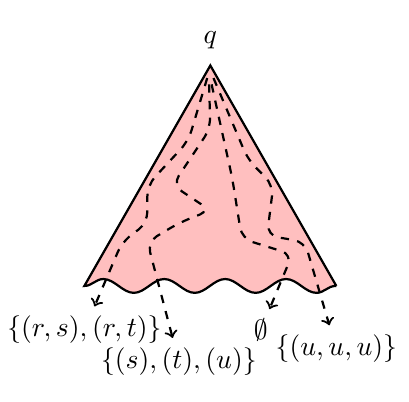
\begin{tikzpicture}
[]
\useasboundingbox (-2.9,-4.9) rectangle (2.7,0.6);

<<<<<<< HEAD
=======

>>>>>>> fcad047018e021c44f6be41eab656d5ec3da0ca5
%\draw[thick,fill=blue!40] (3,-5) -- (0,0) -- (-3,-5) .. controls (-1,-3.5) and (1,-6.5) .. (3,-5);
\draw[thick,fill=pink] (2,-3.5) -- (0,0) -- (-2,-3.5) decorate[decoration=snake,segment length=22] { -- cycle};

\node at (0,0.4){$q$};

\node(set1) at (-2,-4.2) {$\{(r,s),(r, t)\}$};
\node(set2) at (-0.5,-4.7) {$\{(s), (t), (u)\}$};
\node(set3) at (0.8,-4.2) {$\emptyset$};
\node(set4) at (2,-4.5) {$\{(u, u, u)\}$};

\draw[->,thick,dashed,rounded corners] (-0.05,-0.2) -- (-0.35,-1.2) -- (-1,-1.9) -- (-1,-2.5) -- (-1.4,-2.8) -- (set1);
\draw[->,thick,dashed,rounded corners] (-0.02,-0.3) -- (0,-1) -- (-0.6,-1.9) -- (0,-2.3) -- (-0.5,-2.5) -- (-1,-2.8) -- (set2);
\draw[->,thick,dashed,rounded corners] (0.02,-0.3) -- (0.35,-1.8) -- (0.5,-2.75) -- (1.3,-3) -- (set3);
\draw[->,thick,dashed,rounded corners] (0.05,-0.2) -- (0.6,-1.5) -- (1,-1.9) -- (0.9,-2.7) -- (1.5,-2.8) -- (set4);



\end{tikzpicture}
		\caption{MTBDD Top-down representation of a NTA. Image is taken from \cite{tacas12}.}
		\label{fig:mtbdd_td}
	\end{subfigure}%
	~
	\begin{subfigure}{.5\textwidth}
	\centering
	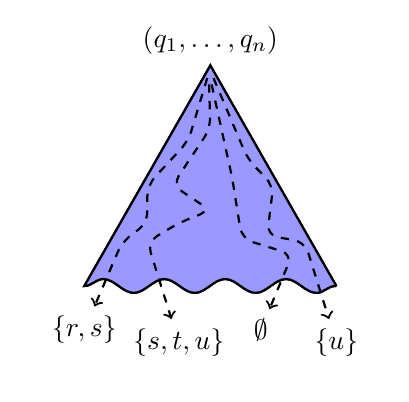
\begin{tikzpicture}
[]
\useasboundingbox (-2.9,-4.9) rectangle (2.7,0.6);
<<<<<<< HEAD
%\draw[thick,fill=blue!40] (3,-5) -- (0,0) -- (-3,-5) .. controls (-1,-3.5) and (1,-6.5) .. (3,-5);
\draw[thick,fill=blue!40] (2,-3.5) -- (0,0) -- (-2,-3.5) decorate[decoration=snake,segment length=22] { -- cycle};

=======

%\draw[thick,fill=blue!40] (3,-5) -- (0,0) -- (-3,-5) .. controls (-1,-3.5) and (1,-6.5) .. (3,-5);
\draw[thick,fill=blue!40] (2,-3.5) -- (0,0) -- (-2,-3.5) decorate[decoration=snake,segment length=22] { -- cycle};


>>>>>>> fcad047018e021c44f6be41eab656d5ec3da0ca5
\node at (0,0.4){$(q_1,\dots, q_n)$};

\node(set1) at (-2,-4.2) {$\{r,s\}$};
\node(set2) at (-0.5,-4.4) {$\{s, t, u\}$};
\node(set3) at (0.8,-4.2) {$\emptyset$};
\node(set4) at (2,-4.4) {$\{u\}$};

\draw[->,thick,dashed,rounded corners] (-0.05,-0.2) -- (-0.35,-1.2) -- (-1,-1.9) -- (-1,-2.5) -- (-1.4,-2.8) -- (set1);
\draw[->,thick,dashed,rounded corners] (-0.02,-0.3) -- (0,-1) -- (-0.6,-1.9) -- (0,-2.3) -- (-0.5,-2.5) -- (-1,-2.8) -- (set2);
\draw[->,thick,dashed,rounded corners] (0.02,-0.3) -- (0.35,-1.8) -- (0.5,-2.75) -- (1.3,-3) -- (set3);
\draw[->,thick,dashed,rounded corners] (0.05,-0.2) -- (0.6,-1.5) -- (1,-1.9) -- (0.9,-2.7) -- (1.5,-2.8) -- (set4);



\end{tikzpicture}
	\caption{MTBDD Bottom-up representation of a NTA. Image is taken from \cite{tacas12}.}
	\label{fig:mtbdd_bu}
	\end{subfigure}%
\end{figure}
\endgroup

Another already implemented encoding is semi-symbolic based on VATA own implementation of MTBDD package.
This encoding is efficient mainly for TA with large alphabet.
Because semi-symblic encoding and MTBDD are not in the aim of this thesis the will no be detaily described
but it is possbile to find such kind of description in \cite{lengal10}.
The main idea of semi-symbolic encoding is shown in Figure \ref{fig:symnta}.
First of all it is necessary to distinguish between (a) top-down and (b) bottom-up variants of this encoding.
The first one maps each state $q$ of a NTA using MTBDD to the sets of the tuples of states such that that it is possible
to make transtion from $q$ under a symbol $a$ to a tuple in apropriate set (each set of tuples is dedicated
to one symbol under which it is possible to make transition from $q$ to the tuples in the set).
The former one symetrically maps each n-tuple $(q_1,\ldots,q_n)$ of a NFA using MTBDD to the sets of states
where each set $S$ is dedicated to a symbol $a$ of the NFA and contains states such that there exists a transition
with $(q_1,\ldots,q_n)$ on the right-handed side and symbol $a$ and state from the set $S$ on the left-handed side.
The final state set of a NTA is again represented by explicit set in both variants,
state set is not stored explicitly because one can obtain it from transition relation and
the symbols are encoded (as binary strings) in MTBDD.

All of the mentioned encodings currently support efficient language inclusion checking using algorithm
from \cite{tacas10} but this does not hold for other operations because some of them are not implemented yet for specific encoding.
The full enumeration of the supported operations for the particular encodings is given in Table \ref{tab:vataop}.

\begin{table}[bt]
	\begin{center}
		\catcode`\-=12
		\begin{tabular}{| l | c | c | c |} \hline
		& {\textbf{Explicit}} & \multicolumn{2}{|c|}{\textbf{Semi-symbolic}} \\ \cline{2-4}
		\textbf{Operation} & \textbf{top-down} & \textbf{bottom-up} & \textbf{top-down} \\ \hline
		Union & $+$ & $+$ & $+$ \\
		Intersection & $+$ & $+$ & $+$ \\
		Complement (experimental) & $+$ & $+$ & $+$ \\
		Removing useless states & $+$ & $+$ & $+$ \\
		Removing unreachable states & $+$ & $+$ & $+$ \\
		Simulation & $+$ & $-$ & $-$ \\
		Downward Inclusion  & $+$ & $+$ & $-$ \\ 
		Upward Inclusion  & $+$ & $-$ & $-$ \\ 
		Simulation over LTS (Labeled Transitions System) & $+$ & $-$ & $-$ \\ \hline
		\end{tabular}
	\caption{Table of supported operations over NTA by particular encodings implemented in \vata.
	Table is taken from \cite{bt:hruska}.}
	\label{tab:vataop}
	\end{center}
\end{table}


\section{Forester}
\label{sec:FA}

Forester is open source tool for verification of program manipulation complex dynamic data structures.
It currently supports program in C langauge.
Forester is distributed as a \emph{GCC} plugin under GPL license, version 3, and can be obtained from its official websice \cite{www.:forester}.
Tool is written in C++.

\subsection{Design}

Forester is implemented as a GCC plugin but it does not analyze directly intermediate code of GCC called GIMPLE but is
uses Code Listener infrastructure \cite{codelistnere} to provide fronted over GIMPLE.

To get high level overiview of verification process performed by Forester please see Figure \ref{fig:fa_exec}. 
Forester starts analysis of a program by translation of intermediate code representation provided by Code Listenter
to its own microcode.
Microcode represents each program statement by one or few instruction which are indeed abstract transformers.
Symbolic execution is then execute over this microcode.
Abstract domain represented by TA as the core part of symbolic state is gradually transformed by abstract transformers
represented by the microcode instructions during the symbolic execution.
When Forester detects an error the symbolic execution is aborted and the analyzed program is determined as incorrect one.
When symbolic execution is over Forester checks whether there is no left garbage (ofcourse, garbage is gradually checked also during the symbolic exection)
and if it is not then a shape invariat has been found and the analyzed program is determined as correct.

\begin{figure}[bt]
	\begin{center}
		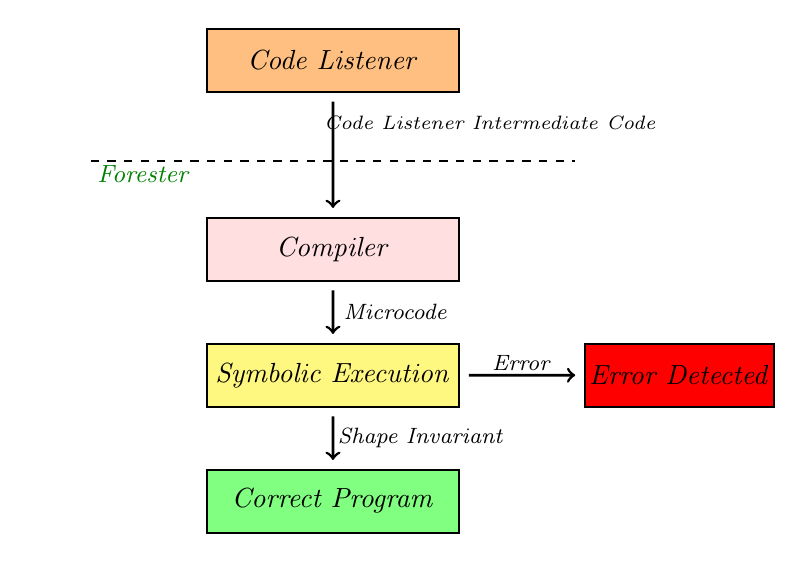
\begin{tikzpicture}[
  cl/.style={thick,fill=orange!50},
  red/.style={thick,fill=Red},
  detection/.style={thick,fill=blue!50},
  compiler/.style={thick,fill=pink!50},
  symexec/.style={thick,fill=yellow!50},
  success/.style={thick,fill=green!50},
  arrow/.style={->,line width=1pt}
  ]

\node (InputNode) at(1.3,10.9) {};
\node (InputDown) at(1.3,10.8) {};

\draw (4,11) rectangle +(4, 1) [cl] node[midway] {\textit{Code Listener}};
\node (CLDown) at(6,11) {};

\draw (4,8) rectangle +(4, 1) [compiler] node[midway] {\textit{Compiler}};
\node (CompUp) at(6,9) {};
\node (CompDown) at(6,8) {};

\draw (4,6) rectangle +(4, 1) [symexec] node[midway] {\textit{Symbolic Execution}};
\node (SymexUp) at(6,7) {};
\node (SymexDown) at(6,6) {};
\node (SymexRight) at(8,6.5) {};

\draw (10,6) rectangle +(3, 1) [red] node[midway] {\textit{Error Detected}};
\node (ErrLeft) at(10,6.5) {};

\draw (4,4) rectangle +(4, 1) [success] node[midway] {\textit{Correct Program}};
\node (CPUp) at(6,5) {};

\draw [arrow] (CLDown) -- (CompUp);
\draw [arrow] (CompDown) -- (SymexUp);
\draw [arrow] (SymexRight) -- (ErrLeft);
\draw [arrow] (SymexDown) -- (CPUp);

\node (LeftFAStart) at(2,9.9) {};
\node (RightFAStart) at(10,9.9) {};
\draw [dashed, line width = 1pt] (LeftFAStart) -- (RightFAStart);

\node (Input) at(8.5,10.5) {\textcolor{Black}{\scriptsize{\textit{Code Listener Intermediate Code}}}};
\node (Input) at(7,7.5) {\textcolor{Black}{\footnotesize{\textit{Microcode}}}};
\node (Input) at(9,6.7) {\textcolor{Black}{\footnotesize{\textit{Error}}}};
\node (Input) at(7.4,5.5) {\textcolor{Black}{\footnotesize{\textit{Shape Invariant}}}};

\node (Input) at(3,9.7) {\textcolor{Green}{\small{\textit{Forester}}}};

\end{tikzpicture}

	\end{center}
	\caption{High level overview of Forester program analysis.}
	\label{fig:fa_exec}
\end{figure}

A little deeper description of conceptual design of Forester (which is shown in Figure \ref{fig:fa_design}) and relations
betweeen its modules will be given now.
Please note that implementation of Forester is not explicitly seprated to the stand-alone compilation modules so the notion of the modules
used in following text is more abstract to provide reader just basic summary of the Forester design.
One module could be e.g. set of closely related classes with a similiar purpose.
As it was mentiond above Code Listener representation of GCC intermediate code is mainly used by Forester \emph{Compiler} module.
Compiler then needs to know \emph{Microcode Instructions} to be able to create their list to run \emph{Symbolic Execution} over it.
Symbolic execcution then execute microcode instructions (abstract transformers) which manipulates \emph{Symbolic State} and of course
also \emph{Forest Automata} included in symbolic states.
Symbolic exection also need \emph{Symbol Context} which is created for each function (and also for global space)
and keeps information about variables used in the function, about function arguments or about stack frame layout.
Symbolic state provides information about state of heap which is represented by FA and it also keeps the information about
corresponding microcode instruction.
\emph{Forest Automata} module provides methods for manipulation FA need during verification procedure.
The operations like normalization or abstraction over FA are not part of module implementing FA implementation but are provided
like stand alone classes which takes FA as parameters.
These operation could be understanded like anothe module \emph{Operation over Forest Automata}.
Finally, Forester currently has its own implementation of \emph{Tree Automata}.
It is very lightweighted implementation containing optimized operations like language inclusion checking using simulation needed for (efficient) Forester run.
The advantage of this implementation is its simplicity and optimization in operation hardly exploited by Forester what makes verification run shorter.
On the other side, it is not easy to mantain such a optimized implementation when one consider that there are still progress in field of design of efficent algorithms
for TA which could bring much higher efficiency then implementation optimization.
\begin{figure}[bt]
	\begin{center}
		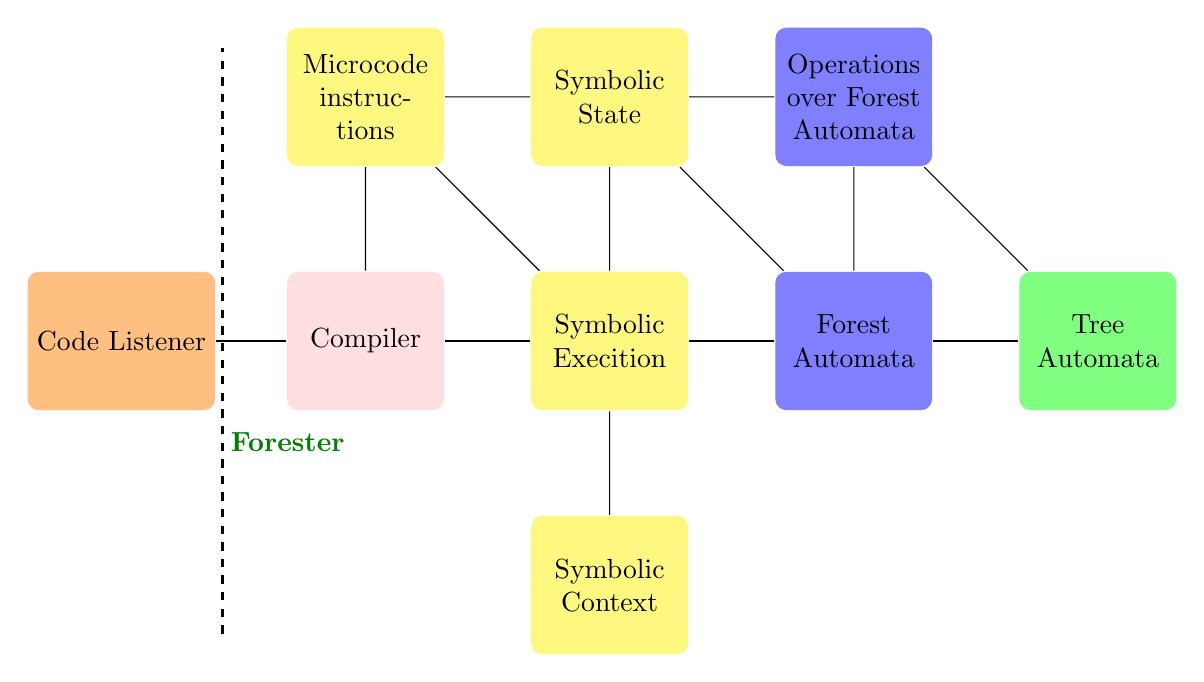
\begin{tikzpicture}[
  scale=0.8,
  node distance = 3.1cm,
  block_cl/.style={rectangle, text centered, rounded corners, thick, fill=orange!50,
    minimum height = 5em, minimum width = 3em},
  block_compiler/.style={rectangle, text centered, rounded corners, thick, fill=pink!50,
    minimum height = 5em, minimum width = 3em, text width = 5em},
  block_symex/.style={rectangle, text centered, rounded corners, thick, fill=yellow!50,
    minimum height = 5em, minimum width = 3em, text width = 5em},
  block_fa/.style={rectangle, text centered, rounded corners, thick, fill=blue!50,
    minimum height = 5em, minimum width = 3em, text width = 5em},
  block_ta/.style={rectangle, text centered, rounded corners, thick, fill=green!50,
    minimum height = 5em, minimum width = 3em, text width = 5em},
  line/.style={draw, -}
  ]

\node [block_cl] (cl) {Code Listener};
\node [block_compiler, right of=cl] (compiler) {Compiler};
\node [block_symex, above of=compiler] (microcode) {Microcode instructions};
\node [block_symex, right of=compiler] (symex) {Symbolic Execition};
\node [block_symex, above of=symex] (symstate) {Symbolic State};
\node [block_symex, below of=symex] (symcnt) {Symbolic Context};

\node [block_fa, right of=symex] (fa) {Forest Automata};
\node [block_fa, above of=fa] (faop) {Operations over Forest Automata};

\node [block_ta, right of=fa] (ta) {Tree Automata};

\path [line] (cl) -- (compiler);
\path [line] (microcode) -- (compiler);
\path [line] (symex) -- (compiler);
\path [line] (symex) -- (symstate);
\path [line] (symex) -- (symcnt);
\path [line] (symex) -- (fa);
\path [line] (symstate) -- (fa);
\path [line] (microcode) -- (symex);
\path [line] (fa) -- (faop);
\path [line] (fa) -- (ta);
\path [line] (symstate) -- (faop);
\path [line] (faop) -- (ta);
\path [line] (microcode) -- (symstate);

\node (LeftFAStart) at(2,-6) {};
\node (RightFAStart) at(2,6) {};
\draw [dashed, line width = 1pt] (LeftFAStart) -- (RightFAStart);
\node (Input) at(3.3,-2) {\textcolor{Green}{\textbf{Forester}}};

\end{tikzpicture}

	\end{center}
	\caption{Conceptual design of Forester.}
	\label{fig:fa_design}
\end{figure}

Please note, that is just concptual high level view of design Forester.
A real implementaion is much more complicated (e.g. Forest automata are implemented by two classes: \emph{FA} and \emph{FAE})
and full technical details.
A full description of the implementation is also not aim of this text and it is not
also possible due to size which could such documentation take.

It was already mentioned that substitution of Forester TA implementation by
VATA could bring some advanteges.
We will summarize them here again.
The first one is fact that it is much easier to maintain one library where
the state-of-the-art algorithms will be implemented and optimized.
Since VATA and Forester is developed by the same developers it also easy to added
to \vata\ operations needed by Forester.
Having narrow interface between TA library and the rest of Forester implementation
also improves code quiality of Forester in the sense of modularity, maintenability and code organization.
These arguments lead us to implement a version of Forester using the VATA library what will be described in chapter \ref{ch:fova}.

\chapter{Forester with VATA}
\label{sec:fova}

This chapter describes process of porting Forester to \vata, its difficulties and design and also deals with implementation
itself.

First of all it is important to declare that we use \vata implementation of explicit encoding of TA because
it is currently the one that support the most of neeeded operations over TA and it is also more efficient than
semi-symbolic encoding for purposes of Forester because no large alphabets are used during verification procedure
so the advantage of the semi-symbolic encoding would not be fully utillizied here.

Forester implementation is currently far from being mature and high structural dependency is
one of its bottlenecks.
So the first thing needed to be done is reducing number of dependencies between classes (described in Section \ref{sec:forester_prep}.
Then it is would be possible to apply design pattern \emph{adapter} \cite{gamma} (described in Section \ref{sec:adapter} to create
interface between Forester and \vata (final implementation described in \ref{sec:fova_impl}.
Applying of adapter design pattern makes possible to include VATA without need of rewriting
Forester to the names of methods and data used in VATA.
It is also creates one place (particularry adapter class) connecting Forester and VATA instead of
including VATA into many of the Forester classes and so it prevents from creating to strong relation between them.

\section{Forester refactoring}
\label{sec:forester_prep}

As it was mentioned there are strong dependencies between classes in Forester implementation.
The original implementation of tree automata library has not been exception so it was needed
to refactore implementation before it would be possible to create adapter clas for \vata API.
The core class of original tree automata is class \emph{TA} and there are also related classes,
e.g. class \emph{TT} for transitions representation or class \emph{Antichain} language inclusion checking using the Antichain algorithm.
This set of classes realizing original tree automata library will be further refered as tree automata module.

The refactoring is mainly based on reduction of the number data types and data members declared
to be \emph{public} (in sense of C++ language).
This is by exploiting features provided by standard C++11 \cite{c++11} which provides methods (keyword \emph{auto})
for auto deduction of the data types by compiler what makes possible to make some of data types of the original tree automata module.
\emph{Iterator} is another concept often used in combination with auto deduction of types to reduce need to export internals of tree automata module.
The combination of these two patterns have been used for example when one needs to iterate over all transitions of tree automata or all transition with some
state as parent.
Another part of refactoring consists simple replacing access of the class data members by corresponding getters and setters method.
Reducing of structural dependencies is also done by emphasis application of \emph{Law of Demeter} \cite{something} what practically
means that classes using TA explicitly should implement methods providing information about TA instead of providing object representing TA itself.
E.g. when one class wants to know whether a given state is final in an tree automaton of an forest automaton then FA implementation should
implement a method instead of providing access to its TA.
Applying the Law of Demeter reduces knowledge needed about implementation of TA module across the whole project what
helps us to make little interface for TA module.
However, Forester coding base is also after this refactoring far from accomplishing mentioned good practice (and also many not mentioned) all around the code.

\section{Adapter design pattern}
\label{sec:adapter}

\emph{Adapter} is structural design patter \cite{gamma} used for creating interface between classes incompatible classes.
Adapter in notion of UML is shown in Figure \ref{fig:adapter}.
Adapter consists from a class \emph{Adaptee} what is the class that we want to make compatible with
another class \emph{Client} which wants to use the methods of Adaptee.
Class \emph{Adaptor} is the one providing connection between Client and Adaptee.
Adaptor could be implemented as inhereted class from Adaptee and employes concept of inheritence to redirect
method calls to its parent (with some possible preprocessing).
Another possible implementation is composing Adaptee to Adaptor and using Adaptor like interface to Adaptee.
Adaptor also could add a new method that combines Adaptee methods to achieve wanted operations.

\begin{figure}
	\begin{center}
		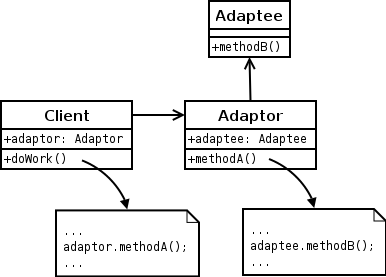
\includegraphics[scale=0.5]{fig/adapter.png}
	\end{center}
	\caption{Adapter design pattern expressed in UML.
	Picture is taken from \cite{wikihttp://en.wikipedia.org/wiki/Adapter_pattern}}
	\label{fig:adapter}
\end{figure}

Let show what are the mentioned roles in our case.
Adaptee is API of \vata, specifically it is class \emph{ExplicitTreeAut} representing a tree automaton in explicit encoding.
Client is not in our case just one class but it is a set of the Forester classes using somehow TA library
and Adaptor is newly implemented class \emph{VATAAdapter} which description is in the following section.

\section{Implementation}
\label{sec:fova_impl}

The main part of adapter design patter is in our case newly implemented class \emph{VATAAdapter} playing role of Adaptor.
We decided to used the implementation approach to Adapter preffering composition over inheritence
because it is more suitable for our purposes since we often needs to rename methods 
(name of a method in Forester differs with name of a method in VATA performing same operation)
or conversion of paremeters data type (e.g. from vector to set). 

So class \emph{VATAAdapter} instantiates class \emph{ExplicitTreeAut} from VATA as its private data member
and redirect to this instance method calls from Forester (the names of methods of VATAAdapter are the same as they were
in the original TA library).
\emph{VATAAdapter} also sometimes performs mentioned data types conversion.
There are also methods implemented by adapter not presented in VATA like method \emph{unfoldAtRoot}
performing some kind of an unfolding.
The methods of this kind are very Forester specific so it is not sensible to add them to general purpose library like \vata is.

We initialy supposed that it will be possible to keep the original TA module with VATA library
to be able easily switch between them.
However it has proved that this would bring high overhead in some sitatuin when a conversion of some data types is needed
compared to situation when there are used directly data types compatible with \vata in Forester code
so we decided to remove the original tree automata module and further support only version of Forester with \vata.

\chapter{template$<$class Text$>$ Backward Run in Forest Automata Based Verification(Text text)}
\label{ch:backward}
text

\section{Backward Run over Symbolic Context}

\section{Intersection of Forest Automata}

\chapter{template$<$class Text$>$ Implementation(Text text)}
\label{ch:impl}
text

\section{Execution Trace}
\section{Module For Intersection}

\chapter{template$<$class Text$>$ Evaluation(Text text)}
\label{ch:eval}
text

\chapter{template$<$class Text$>$ Conclusion(Text text)}
\label{ch:concl}
text
